%--------------------------------------------------------------------------
% !TEX root = 5Blman.tex
% interfere.tex
%--------------------------------------------------------------------------
\chapter{Interference and Diffraction}

\begin{multicols}{2}
%---------------------------------------------------------------------
\section{Purpose}  The purpose of these laboratory exercises is to give you hands-on experience with interference and diffraction effects produced by a double slit.
\section{Preparation}  Reread the section on interference and diffraction before coming to lab.  Pay particular attention to the conditions that produce constructive and destructive interference for light passed through a double slit.  We will also see evidence of single slit diffraction in the double slit pattern, so you should reread the relevant sections and carefully examine the figures in your text associated with the phenomena.

%\begin{wrapfigure}[7]{r}[0pt]{2cm}	
%  \centering
%  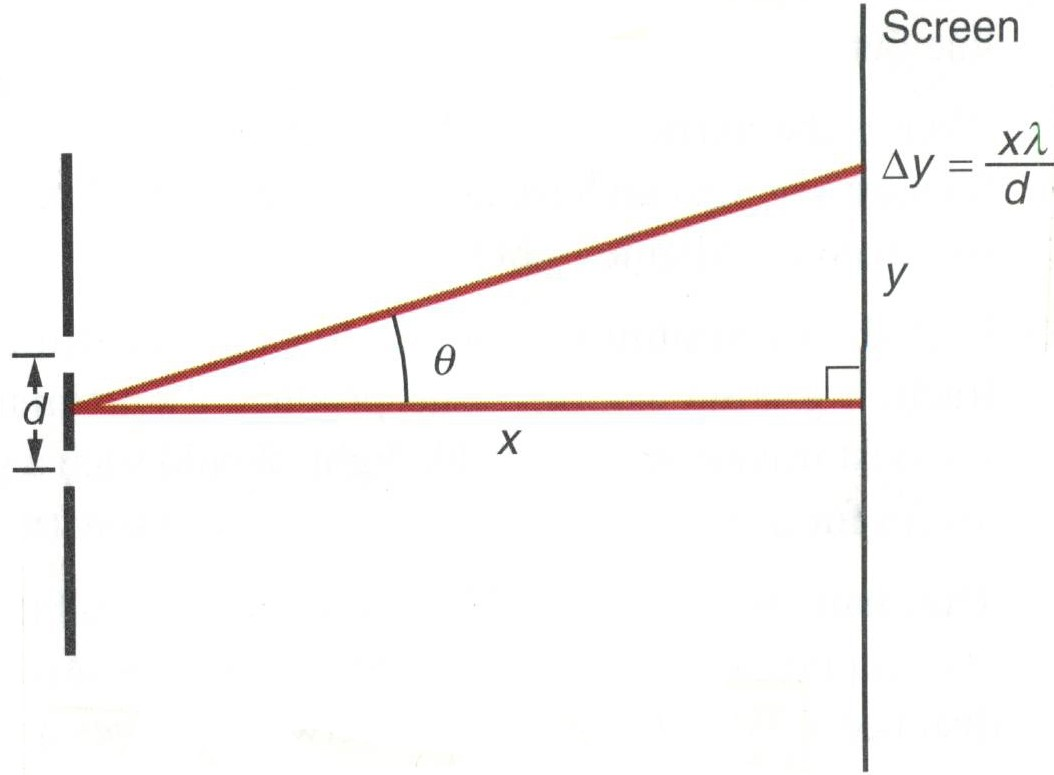
\includegraphics[scale=0.7]{5bgraf/fig_18}
%%  \caption{Double slit interference}
%  \label{f:fig18}
%\end{wrapfigure}

%%\begin{figure}
%\begin{SCfigure} % use sidecap pkg
%	\centering
%	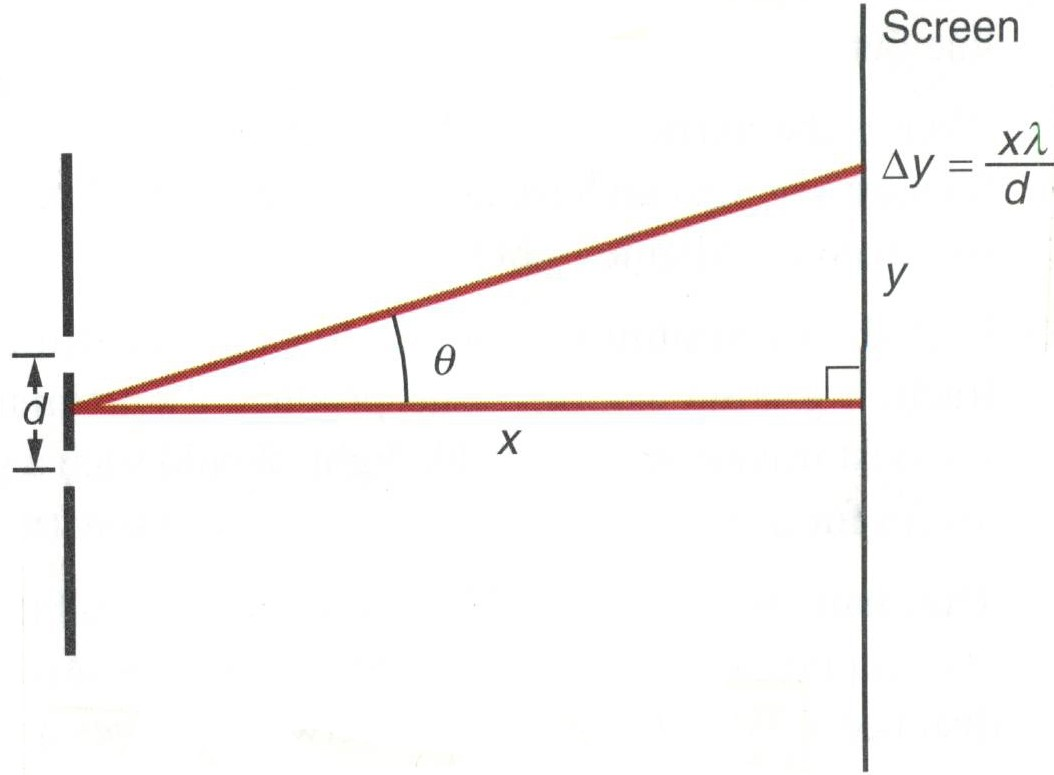
\includegraphics[scale=0.8]{5bgraf/fig_18}
%	\caption{Double slit interference}
%	\label{f:fig18}
%\end{SCfigure}
%%\end{figure}

\begin{center}
	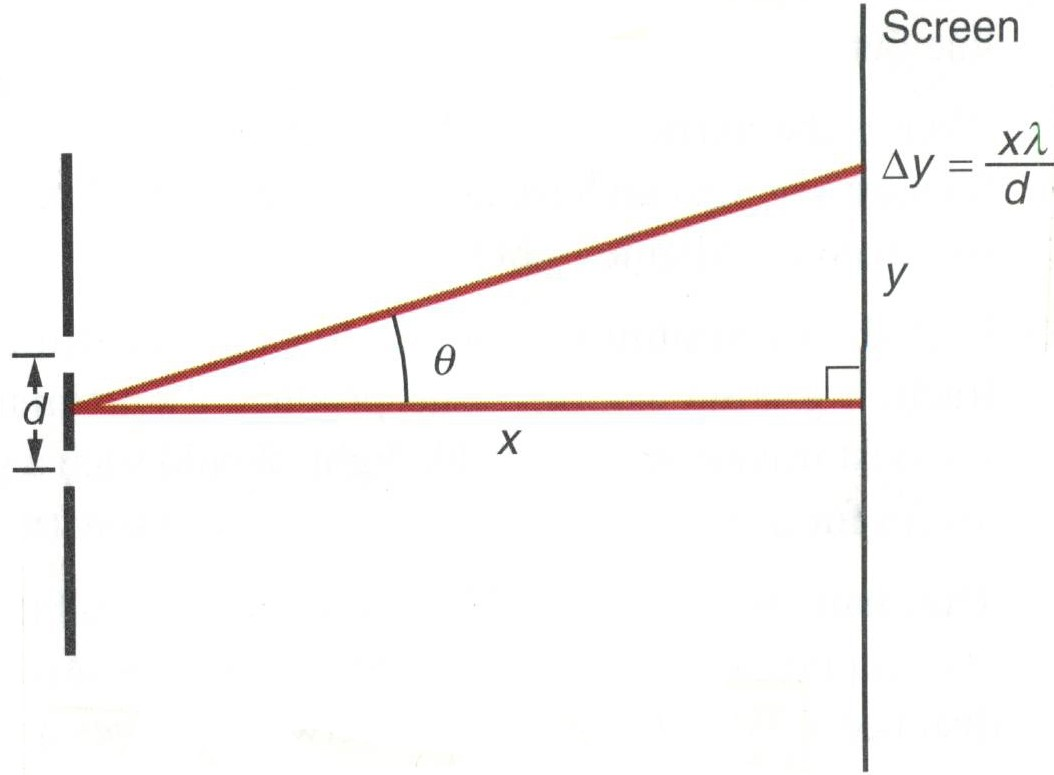
\includegraphics[scale=0.8]{5bgraf/fig_18}
	\mfcaption{Double slit interference}
	\label{f:fig18}
\end{center}

%---------------------------------------------------------------------
\section{General Information}
The figure shown is a schematic of the experimental set up for this laboratory exercise. There is a double slit at a distance $x$ from a screen.  When laser light is shown through the slit toward the screen a diffraction pattern will be observed.  Since the separation of the slits $d$ is relatively large compared to the wavelength  of the light used, there are a large number of bright dots where constructive interference occurs.  These are sometimes referred to as fringes.  Distance along the line of fringes is denoted by $y$. By using a little trigonometry and the small angle approximation, you find that the average distance between fringes under these circumstances is given by: 
\begin{equation} \label{e:deltay}
	\Delta y \approx x  \cdot \frac{\lambda}{d}
\end{equation}

You will measure $\Delta y$, $x$, and $d$ and (\refeqn{e:deltay}) to calculate a value for the wavelength $\lambda$ of a Helium Neon or diode laser. By rearranging the equation above you get:
\begin{equation} \label{e:lambda}
	\lambda \approx d \cdot \frac{\Delta y}{x}
\end{equation}

%---------------------------------------------------------------------
\section {Double slit interference}

\subsection{Activity: Double slit}
% Measure $d$, the double slit separation 
\begin{enumerate}
	\item Your instructor will guide you in adjusting the traveling microscope.  Make at least two measurements of $d$ for each of the double slits you use.  Estimate and record the experimental uncertainty in $d$.
	\item 	Mount the laser and double slit so that a diffraction pattern is produced on a wall at least 4 meters away.  Measure this distance (this is your experimental value of $x$) as accurately as you can.  As usual, estimate and record the uncertainty in this distance.
\end{enumerate}

\subsection{Activity: Wavelength of laser light}
% Record and measure the pattern of fringes
\begin{enumerate}
	 \item 	Place a piece of paper on the wall and record the location of as many fringes as possible.  Obtain the most accurate value possible for the average distance between fringes.  This is your experimental value of $y$.  Also estimate the uncertainty in your value of $y$.
	 \item Use (\refeqn{e:lambda}) above to calculate the wavelength of light used in this exercise.
	 \item Repeat the process for a second double slit having a different value of $d$.
	 \item Compare your results with the actual value for $\lambda$
	Calculate the percent difference between each of your experimental values for $\lambda$ and the actual value of 632.8 nm for a HeNe laser. The value for a diode laser will differ slightly.
	\item Determine if your experimental results agree with the actual value
	Calculate the percent uncertainties in $y$, $x$, and $d$ based on your estimated uncertainties.  Add the percent uncertainties and see if they are greater than the percent difference between your experimental value and the actual value.  Discuss whether or not you have agreement.
\end{enumerate}

%---------------------------------------------------------------------
\section{Activity: Single slit diffraction}
% Evidence of a single slit diffraction pattern in the double slit pattern
	Describe the evidence for single slit diffraction observed in the double slit pattern.

\section {Conclusions} What evidence did you see for the wave nature of light in today's experiment?  Did your results agree quantitatively or only qualitatively with theory?
 
\end{multicols}
%--------------------------------------------------------------------------
\endinput
%--------------------------------------------------------------------------
